\chapter{Detailed Design}\label{chap:design}

This section presents the detailed greenhouse design using a structured approach: for each design element, requirements are defined first, followed by technical specifications and implementation details. A key design priority is the roof vent to maximize passive ventilation, which guided the geometry and mechanism choices that follow. Following design reviews, a revised structural design was developed to enable improved operation and manufacturability. The general shape was optimized to accommodate laser cutting processes, with the use of the universities CO2 laser cutter with a maximum available bed size of \SI{1260}{mm} $\times$ \SI{860}{mm}. The roof geometry was modified to an uneven-span lean-to configuration. While this maintains a steep roof inclination for efficient solar gain, it also allows for better thermal control and ensures that the roof vent can be actuated even when the greenhouse is positioned adjacent to a wall.

Allowing users to place the greenhouse against a thermally massive surface (e.g., a concrete or brick wall) enhances passive heat retention and improves overall energy performance. Additionally, the revised structure introduced more right angles, simplifying manufacturing and increasing the usable internal volume of the greenhouse.

\begin{figure}[h]
	\centering
	\begin{subfigure}[b]{0.43\textwidth}
		\centering
		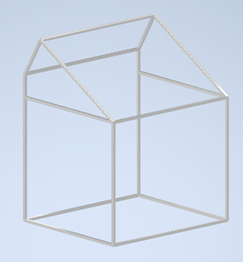
\includegraphics[width=\textwidth]{figs/frame.png}
		\caption{Frame Structure}
		\label{fig:image1}
	\end{subfigure}
	\hspace{0.6em} % was \hfill — make this small; 0pt to touch, negative to overlap
	\begin{subfigure}[b]{0.41\textwidth}
		\centering
		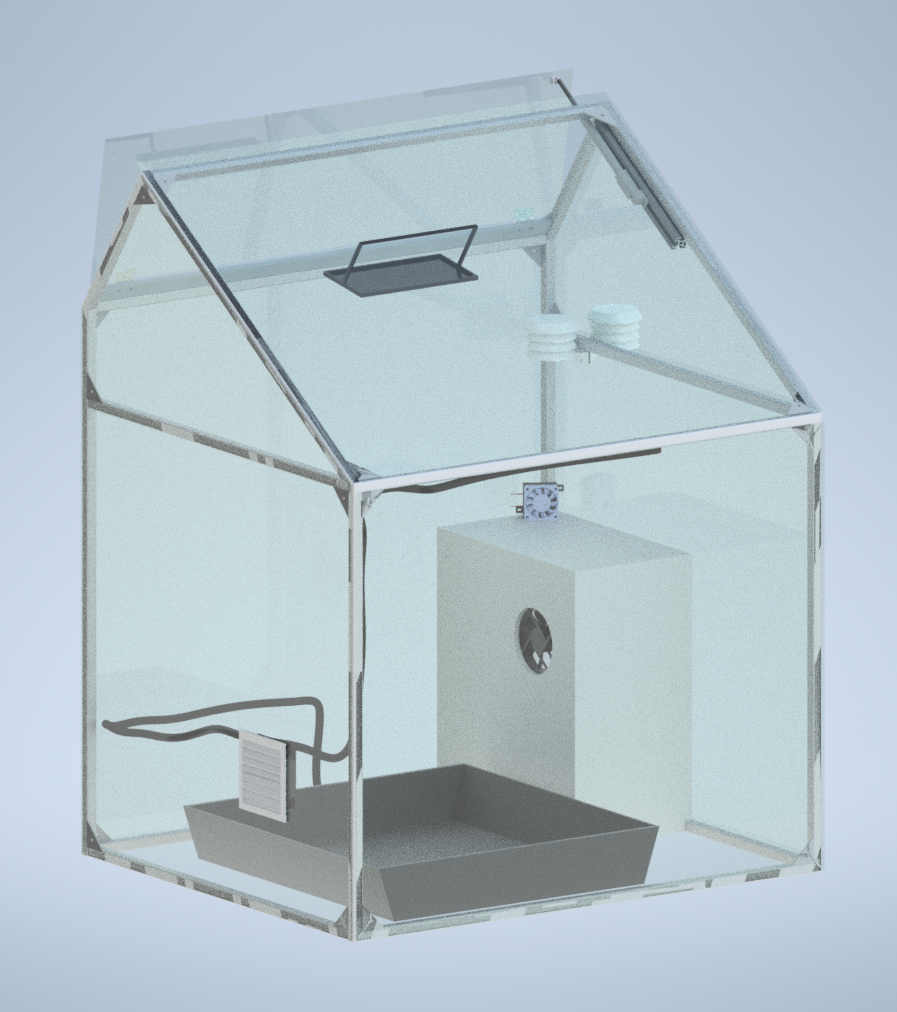
\includegraphics[width=\textwidth]{figs/front.png}
		\caption{Final Concept}
		\label{fig:image2}
	\end{subfigure}
	\caption{Detailed Design}
	\label{fig:side_by_side}
\end{figure}

\begin{figure}[H]
	\centering
	\fbox{\includegraphics[width=0.86\textwidth]{figs/anotated.png}}
	\caption{Final Concept Definition}
	\label{fig:Final_concept}
\end{figure}

The control center protecting all of the electrical components is shifted to the side of the greenhouse and a door is laser cut from the right side Perspex panel allowing easy access for maintenance. This side access preserves the ability to have the greenhouse be leveraged against an existing wall maximizing space efficiency. Hinges on the front Perspex panel enable it to open for convenient access required for planting and harvesting.


\section{Structure}
\subsection{Frame}
The frame must provide a durable structural foundation that supports the greenhouse covering material, withstands environmental loads such as wind and rain, and does so in a cost-effective manner. Aluminum square tubing is selected for its excellent strength-to-weight ratio. Compared to a stainless steel frame, aluminum offers a much lighter structure, making the greenhouse easier to transport or reposition if necessary. Additionally, aluminum is naturally corrosion-resistant, eliminating the need for protective coatings to prevent rust. Standard aluminium extrusions are also widely available and relatively easy to cut and assemble, making it a practical and cost-effective choice for the frame. A structural analysis seen in the calculations in Appendix \ref{chap:calcs} confirmed that the frame can withstand its own weight, the weight of Perspex panels, and wind loads simultaneously. The calculated safety factor for the aluminium frame, based on maximum wind loads of up to 40 km/h acting perpendicularly to the side panels, was determined to be approximately 40.1 . The maximum deflection simulated at the apex of the greenhouse amounted to only 0.5\,mm, demonstrating excellent structural stiffness and integrity. Detailed engineering drawing of the frame assmbly can be seen in Appendix \ref{fig:engineering-drawing}

\subsection{Covering material}
Perspex was chosen over glass for its combination of machinability, thermal performance, transparency, and non-brittle nature, addressing both construction and long-term durability needs.

\section{Control Center Design}
\subsection{Electrical Component Housing}
A dedicated area is required for the safe and neat storage of all electrical components such as the battery, charge controller, buck convertor, microcontroller, relays and valve. The control center can be made from wood as it is simple to construct and mount parts to, as well as being electrically nonconductive and thermally insulating. Specifically, marine plywood is used as it resists water damage and is made from high-quality hardwood veneers, making it stronger and more resistant to warping compared to standard plywood. Coating it with white exterior-grade paint will further improve water resistance and reflect sunlight, keeping internal components cooler while reflecting more light for the plants. Silicone sealant is applied in and around the control centre to ensure waterproofing and isolate it from the greenhouse environment, protecting components from misting and rain.

\begin{figure}[H]
	\centering
	\fbox{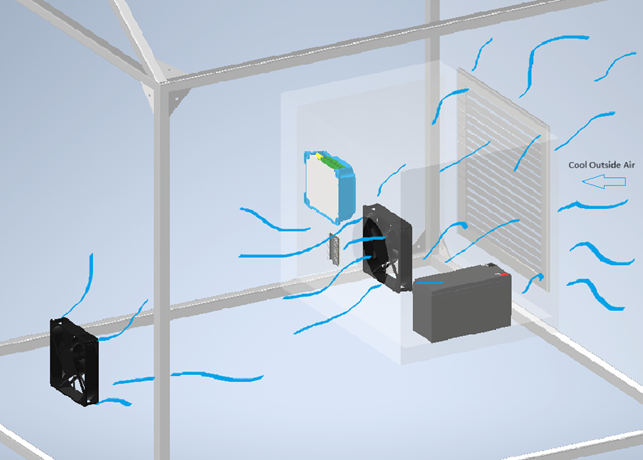
\includegraphics[width=0.65\textwidth]{figs/airflow1.png}}
	\caption{Air Intake}
	\label{fig:air_circulation}
\end{figure}

\subsection{Control Center Ventilation }
A cutout from the Perspex allows for placement of a louvre vent as seen in figure \ref{fig:air_circulation}. These vents will allow for passive ventilation to keep the control center cool while the shape of the louvre vents will prevent water from entering. This vent is placed on the side of the greenhouse to allow for the placement of the greenhouse against a wall. 

For this reason, the control center was moved to the right side of the greenhouse, freeing up more space for plants. Dedicated ventilation prevents overheating, a strategically positioned HAF fan mounted on the enclosure's side creates an airflow path drawing outside air through the large louvred vent, across the electronics, and exhausting it into the greenhouse. This dual-purpose setup cools the control and electrical components while supplying fresh air to the growing environment.

\subsection{Access Panel}
A cutout from the side panel around the control center allows for the placement of a door providing easy access to the electrical components. This door will also incorporate the louvred vent, enabling proper ventilation for the electrical components and acting as the intake for the HAF fan attached to the side of the control center.

\section{Intake and HAF fans}
Intake fans bring in fresh oxygen rich air when needed. To regulate the greenhouse temperature, cool air is drawn in from the base while a top vent opens to allow warm air to escape, promoting natural convection and effective cooling. Industrial greenhouses also rely on HAF fans to promote healthy air movement and prevent stagnation. However, on a smaller scale, dedicated HAF fans are not necessary. For the sake of simple design and using smart controller logic these two actions of air intake and HAF can be combined to be completed by the same two components. In this case two 12V fans on either side of the greenhouse are placed towards the bottom section of the greenhouse. These two fans will allow for air intake when necessary as well as intermediate HAF control at set intervals. The fans are placed slightly offset from each other to promote circular airflow and improve coverage.

\begin{figure}[H]
	\centering
	\fbox{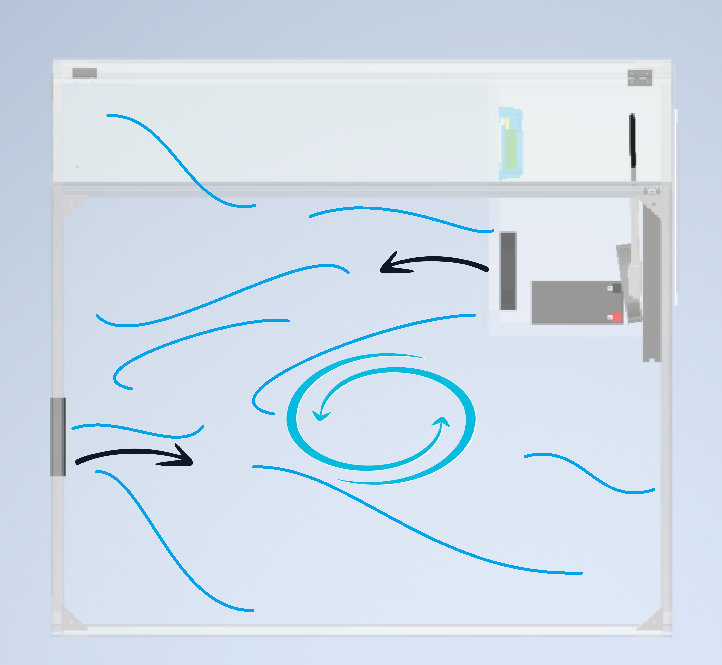
\includegraphics[width=0.5\textwidth]{figs/whirlpool.png}}
	\caption{Air circulation}
	\label{fig:air_circulation}
\end{figure}

Exhaust fans were excluded from the design as the roof vent, having a large surface area, will allow for the escape of a large quantity of air when the air intake and ventilation is active. This exhaust flow is assisted by the buoyancy effect as stipulated in the calculations in Appendix \ref{chap:calcs}

\subsection{HAF Requirements}

A common guideline is to size the HAF fans to be able to move 2 CFM for each square foot of greenhouse floor area \citep{Watson2019}. By these standards for the floor area of 0.85\,m\textsuperscript{2} an HAF capacity of at least 18.3\,CFM would be required to ensure healthy air circulation. Two 120\,mm PC fans with an average of 70\,CFM each will be more than sufficient and will be activated during dedicated HAF periods.

\begin{align}
	\small
	A_{\text{floor}} &:= b \cdot l = 0.85 \,\si{m^2} \\[1em]
	A_{\text{floor,ft}} &:= A_{\text{floor}} \cdot 10.764 \,\frac{\si{ft^2}}{\si{m^2}}
	= 9.1494 \,\si{ft^2} \\[1em]
	CFM_{\text{HAF}} &:= A_{\text{floor,ft}} \cdot 2 \,\frac{\si{ft}}{\si{min}}
	= 18.2988 \,\frac{\si{ft^3}}{\si{min}}
\end{align}

Due to the use of misting systems within the greenhouse care needs to be taken to protect the fans and other components from moisture buildup, for this reason 3D printed covers and louvered vents are designed to protect from droplet buildup on components. Smart placement of misting nozzles and intermediate misting control will also prevent excessive moisture exposure to electrical components.

\section{Ventilation}

\subsection{Natural Ventilation}

An effective ventilation system at the top of the greenhouse will allow for passive cooling using the buoyancy effect of the warm air within the greenhouse. The larger the area of the vent the more effective the air transfer and thus cooling capabilities. A Perspex panel on the roof measuring 1000mm by 270mm is to be actuated to the open position to allow for this exchange. A linear actuator is selected as it is less complicated than installing a motor and shaft and more cost effective. The actuator selected should have a large stroke of at least 100mm to increase the opening area and will need to be rated to lift the weight of the Perspex panel. Calculations seen in Apendix \ref{chap:calcs} were completed to ensure that the specification can be met and an example can be seen in the free body diagram below. 

\begin{figure}[H]
	\centering
	\fbox{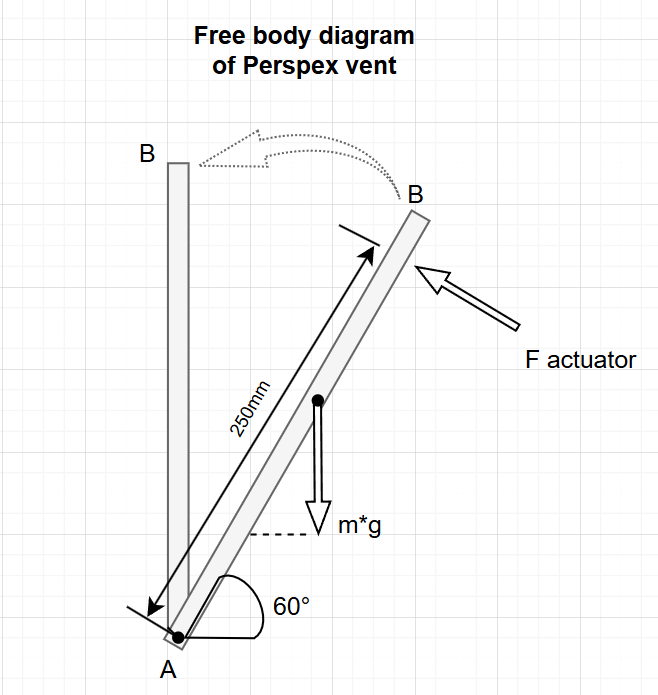
\includegraphics[width=0.3\textwidth]{figs/fbd.png}}
	\caption{Free body diagram of Vent Mechanism}
	\label{fig:vent_fbd}
\end{figure}

When opened, the vent exposes the greenhouse interior to potential precipitation, which could result in overwatering or water exposure to electrical components. To mitigate this, a rain sensor is mounted on the exterior of the greenhouse and connected to the microcontroller. When moisture is detected, the sensor signals the system to close the vent, thereby protecting both the plants and internal electrical components during periods of rain.

\subsection{Forced Ventilation}
 
Typical greenhouse design guidelines recommend approximately one complete air exchange per minute \citep{Watson2019}. With a greenhouse volume of 0.77~m$^3$, this requires two fans with a combined flow rate of at least 0.77~m$^3$/min. Calculations in Appendix \ref{chap:calcs} indicate that the volumetric flow rate of the intake fans must be at least 27~CFM. Accordingly, two PC fans, each averaging 70~CFM, are selected, more than sufficient to exchange the entire greenhouse volumes air within one minute.

\section{Misting System}

Effective greenhouse environmental control requires regulating soil moisture while maintaining relative humidity (RH) within crop-specific setpoints. To avoid the complexity of parallel systems, this design adopts a single misting system coordinated by scheduling and control procedures to handle both irrigation and humidity management. When irrigation or a misting cycle elevates RH, the mechanical ventilation is automatically engaged to exhaust excess moisture and restore RH to the target range. The developed control algorithms for this optimization can be seen in appendix \ref{flow}. A further advantage of the misting system is evaporative cooling, which operates in combination with the greenhouse’s passive (roof vent) and active ventilation to limit temperature spikes above desired thresholds.

Misting Nozzles are placed effectively to ensure moisture reaches the roots directly. Up to 4 nozzles are placed slightly above the soil and deliver water straight to the soil medium. Misting nozzles offer adjustable spray patterns, ranging from a targeted drip to an ultra-fine mist. Two additional nozzles will be installed at a higher elevation within the greenhouse to provide broader coverage while still targeting specific zones. Careful positioning will ensure mist is directed away from sensitive electrical components. 

\section{Active Heating System}
To achieve effective active heating, a fan heater is selected. Based on the heat loss calculations on the surface area, the greenhouse experiences a convective heat loss of approximately 119\,W when there is a 5\,°C temperature difference between the internal and external environments. 

Given that many plants require a minimum desirable temperature of around 15\,°C for optimal growth, the heating system must be capable of compensating for this heat loss. Therefore, a fan heater with a power rating of at least 120\,W is required.

A 12,V, 120,W fan heater is provided by the university to meet this requirement, powered directly by the 12,V battery supply. The heater is controlled via a relay module, which is switched by signals from the microcontroller. This setup allows the heater to automatically activate when the internal temperature falls below a user-defined threshold. A hysteresis band is implemented in the code, this prevents fast unnecessary switching, allowing for accurate feedback and extending the lifespan of the heater and relays.


\section{Environmental Monitoring}
\label{sec:environmental_monitoring}
The greenhouse uses a network of environmental sensors connected to a central microcontroller to continuously monitor key parameters such as temperature, humidity, soil moisture, light intensity, and CO\textsubscript{2} concentration. These measurements provide real-time feedback on the internal climate conditions, which are essential for optimizing plant health and growth. 

The data collected is processed by the microcontroller and used both for local decision-making (e.g., activating ventilation or irrigation systems) and for remote monitoring via IoT platforms. Through cloud-based interfaces, users can access historical data and current conditions, and adjust system settings as needed. The following sections detail the selection and implementation of the microcontroller, the individual sensors, and the data acquisition platforms used in the system.

\subsection{Controller}
\label{subsec:controller}
The ESP32 microcontroller, developed by Espressif, is selected for its abundant I/O options, making it ideal for managing multiple sensors and actuators through its numerous GPIO pins. Its built-in Wi-Fi and Bluetooth connectivity enables seamless communication with user interfaces, allowing for real-time monitoring of the greenhouse environment.

The ESP32 supports a variety of communication protocols such as I\textsuperscript{2}C, UART, and SPI, allowing seamless integration with environmental sensors and control modules. Its dual-core processing power ensures efficient real-time data handling and decision-making. Its integration with Arduino's IDE software allows for easy programming capabilities. Additionally, the ESP32's low power consumption and wide community support make it a reliable and cost-effective choice for an embedded greenhouse controller.

\subsection{Sensors}
\label{subsec:sensors}
Multiple sensors enable accurate monitoring of both the internal greenhouse environment and the external ambient conditions. This data informs the control of greenhouse parameters and provides a baseline for comparison between internal and external climates. 

The external temperature and humidity sensor will be exposed to direct sunlight and rainfall, while the internal sensors will experience both sunlight and periodic misting. To ensure longevity and reliable performance, protective housings are required. Custom 3D-printed Stevenson screens can shield sensors from water and heat while allowing airflow through their slatted design for accurate readings. White filament is recommended to reflect sunlight and minimize heat absorption. In accordance with standards, the Stevenson screen should be mounted around 1.2m above ground level~\cite{manclim}.

\begin{figure}[htbp]
	\centering
	\fbox{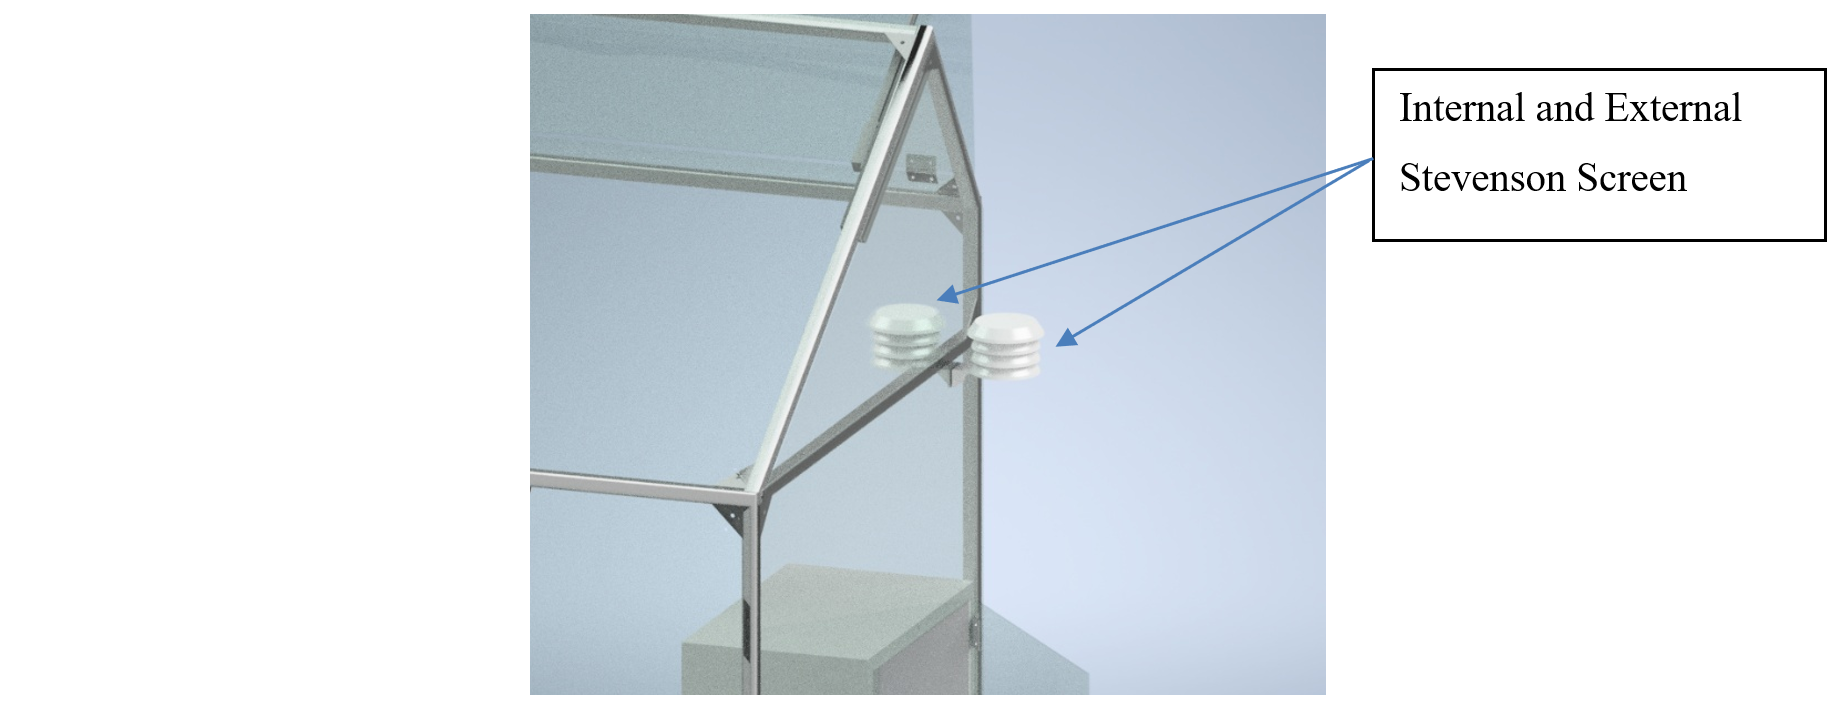
\includegraphics[width=0.9\textwidth]{figs/steven.png}}
	\caption{Stevenson Screens for sensor protection}
	\label{fig:stevenson_screens}
\end{figure}

The following sections break down each sensor's selection and operation.

\subsubsection{ Temperature and Humidity Sensor}

The DHT22 sensor was selected for its balance of accuracy, low cost, and ease of integration. Since it measures both temperature and relative humidity, it reduces the need for separate sensors, streamlining wiring and system design. It communicates with the ESP32 using a single-wire digital interface, making implementation straightforward.

\begin{table}[H]
	\centering
	\caption{DHT22 Temperature and Humidity Sensor Specifications}
	\label{tab:dht22_specs}
	\begin{tabular}{ll}
		\toprule
		\textbf{Parameter} & \textbf{Specification} \\
		\midrule
		Temperature Range & -40 to 80\,$^\circ$C \\
		Temperature Accuracy & $\pm$0.5\,$^\circ$C \\
		Humidity Range & 0--100\,\% RH \\
		Humidity Accuracy & $\pm$2--5\,\% RH \\
		Operating Voltage & 3.3--5.5\,V \\
		Output Signal & Digital (single-wire protocol) \\
		\bottomrule
	\end{tabular}
\end{table}


\subsubsection{ Light Sensor}
The BH1750 light sensor is chosen for its good balance of accuracy, cost-effectiveness, and ease of integration. It provides precise ambient light measurements in lux, making it suitable for monitoring plant lighting conditions with a simple conversion to PPFD values. It’s I²C communication protocol allows seamless and reliable connection with the ESP32, using only two GPIO pins. The sensor also requires minimal configuration and is supported by well-documented libraries, enabling quick setup and consistent performance in greenhouse environments.

\begin{table}[h]
	\centering
	\caption{BH1750 Light Sensor Specifications}
	\label{tab:bh1750_specs}
	\begin{tabular}{ll}
		\toprule
		\textbf{Parameter} & \textbf{Specification} \\
		\midrule
		Operating Voltage & 3.3-5V \\
		Interface & I\textsuperscript{2}C (7-bit address: 0x23 or 0x5C) \\
		Measurement Range & 1--65,535\,lx \\
		Resolution & 1\,lx (High-Resolution Mode) \\
		Accuracy & $\pm$20\% at 25$^\circ$C \\
		Current Consumption & $\approx$0.12\,mA (active), 0.01 \\
		\bottomrule
	\end{tabular}
\end{table}


\subsubsection{ Carbon Dioxide Sensor}
The MH-Z19 CO\textsubscript{2} sensor is chosen due to its balance of affordability, accuracy, and ease of integration with microcontrollers like the ESP32. It uses Non-Dispersive Infrared (NDIR) technology to detect CO\textsubscript{2} concentrations, which provides reliable and stable readings with minimal calibration necessary.

The sensor communicates through UART or PWM, offering flexibility in how data is read by the system. Its compact design and low power consumption (typically 33\,mA at 5\,V) make it ideal for continuous indoor monitoring in environments such as greenhouses. The sensor has a measurement range of 0--5000\,ppm with an accuracy of ±(50\,ppm + 5\% of reading) in the 0--2000\,ppm range.

\begin{table}[H]
	\centering
	\caption{MH-Z19 CO\textsubscript{2} Sensor Specifications}
	\label{tab:mhz19_specs}
	\begin{tabular}{ll}
		\toprule
		\textbf{Parameter} & \textbf{Specification} \\
		\midrule
		Communication & UART, PWM \\
		Operating Voltage & 3.6--5.5\,V \\
		Current Consumption & 33\,mA (typical) \\
		Measurement Range & 0--5000\,ppm \\
		Accuracy & ±(50\,ppm + 5\% of reading) \\
		Warm-up Time & 3 minutes \\
		\bottomrule
	\end{tabular}
\end{table}


\subsubsection{ Soil Moisture Sensor}
\label{subsubsec:soil_moisture}
The soil moisture sensor needs to provide real-time monitoring of substrate hydration levels, enabling the automated misting system to deliver precise irrigation when needed. A generic industrial grade capacitive soil moisture sensor and module is selected for its simplicity, cost-effectiveness, and compatibility with the ESP32 microcontroller.

\begin{table}[h]
	\centering
	\caption{SEN0114 Soil Moisture Sensor Specifications}
	\label{tab:sen0114_specs}
	\begin{tabular}{ll}
		\toprule
		\textbf{Parameter} & \textbf{Specification} \\
		\midrule
		Output Signal & Analog voltage \\
		Operating Voltage & 3.3--5\,V \\
		Interface & 1-wire (requires ADC) \\
		Probe Material & Corrosion-resistant alloy \\
		Measurement Depth & Up to 37\,mm \\
		\bottomrule
	\end{tabular}
\end{table}

The sensor operates by measuring the conductivity between two exposed probes inserted into the soil, where higher conductivity indicates greater moisture content. It provides an analog voltage output (0--3.3\,V) corresponding to the soil's moisture level, allowing for real-time monitoring of water content in the growing medium. 

The sensors ease of integration and low power requirements (drawing less than 20\,mA) make it well-suited for irrigation automation. The sensor only requires one wire for communication and connects to an analog-to-digital converter (ADC) pin on the ESP32. Initial calibration is required to establish the relationship between voltage output and actual soil moisture content. This can be achieved as follows. 

\subsubsection*{Calibration Procedure}

\begin{enumerate}
	\item \textbf{Hardware Setup:} Connect the soil moisture sensor's output to an ADC compatible pin (e.g., GPIO 11) set to 12-bit resolution on the ESP32. Ensure the sensor is powered correctly.
	
	\item \textbf{Wet Point Calibration:} Place the sensor probes in fully saturated soil (considered 100\% moisture). Record the stable ADC reading, \( R_{\text{wet}} \).
	
	\item \textbf{Dry Point Calibration:} Place the sensor probes in completely dry soil (considered 0\% moisture). Record the stable ADC reading, \( R_{\text{dry}} \).
	
	\item \textbf{Software Implementation:} In the microcontroller code, map subsequent ADC readings (\( R \)) to a percentage value using the following linear interpolation formula:
	
	\begin{equation}
		\text{Moisture Percentage} = \left( \frac{R - R_{\text{dry}}}{R_{\text{wet}} - R_{\text{dry}}} \right) \times 100\%
	\end{equation}
\end{enumerate}

\subsubsection{ Rain Sensor}

A rain sensor is mounted on the exterior of the greenhouse to detect rainfall and trigger protective actions. When rainfall is detected, the system is programmed to automatically close the ventilation openings, thereby safeguarding electrical components and preventing overwatering of the plants. 

The selected model is an HKD general-purpose rain sensor, which features a large sensing surface to improve droplet detection. The sensor operates by using exposed conductive tracks on the board: when water bridges the tracks, the resistance changes significantly, from approximately \SI{2}{\mega\ohm} when dry to around \SI{100}{\kilo\ohm} when wet. This variation is processed by the module, which outputs a digital signal (logic HIGH or LOW) to indicate the presence of rain. 



\subsection{Data Acquisition and Monitoring}
\label{subsec:data_acquisition}


The ESP32 can collect sensor data and store it locally in .xls format on an SD card. However, to provide a more accessible and user-friendly interface, data will instead be uploaded to a cloud-based platform such as ThingSpeak. ThingSpeak supports monitoring and control of up to 8 fields with a minimum update interval of 15 seconds. The free tier offers up to 3 million messages per year, which equates to approximately 8,000 messages per day. Blynk is another free IoT platform that allows for easy creation of mobile apps to control and monitor hardware remotely. It is fully compatible with the Arduino platform, making it a convenient choice for IoT projects. A Blynk dashboard is thus setup alongside a ThingSpeak dashboard to allow for wireless monitoring and control of the greenhouse environment.

\begin{figure}[H]
	\centering
	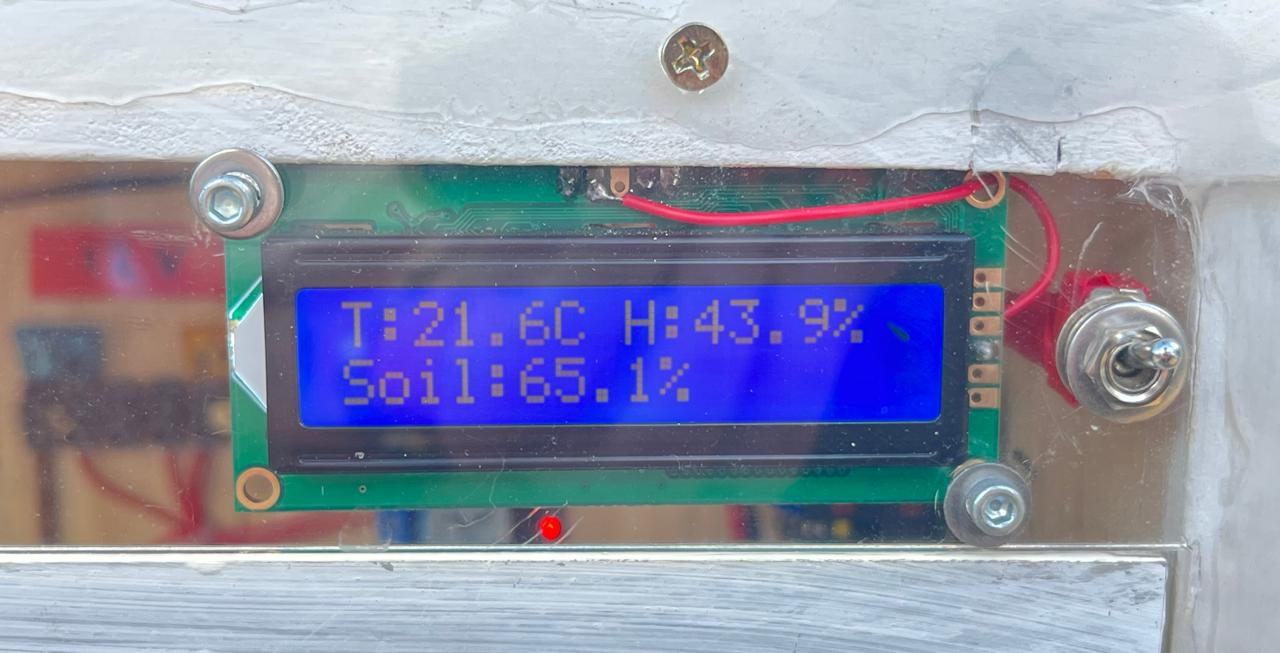
\includegraphics[width=0.5\textwidth]{figs/LCD.jpg}
	\caption{LCD screen for local monitoring}
	\label{fig:lcd_screen}
\end{figure}

\subsubsection*{Local Monitoring}
\label{subsubsec:local_monitoring}
Local monitoring is useful when a user is on-site near the greenhouse and wants to easily view the current internal conditions. Additionally, in the event of a Wi-Fi outage, the greenhouse can still communicate essential data locally. For this reason, a small LCD screen is used to display key environmental parameters, including temperature, humidity, light levels, soil moisture, and CO\textsubscript{2} concentration. The LCM1602A display is selected for its built-in I\textsuperscript{2}C communication interface. 
This allows it to share the same two pins already used by the BH1750 sensor, since I\textsuperscript{2}C supports multiple devices on a single bus through unique addresses. 
The LCM1602A operates at address \texttt{0x3E}, enabling efficient integration while reducing GPIO pin usage compared to the standard 8-bit parallel interface.
The screen cycles through these readings to present the information clearly and efficiently. It is mounted above the control room door and is visible through the Perspex panel, allowing for quick visual access without needing to enter the enclosure. The active screen alongside the all purpose on/off switch can be seen in the figure above.


\section{Power Supply}
\label{sec:power_supply}
The power supply provides energy to the system as a whole and is crucial for the general operation and reliable functioning of the device. Power is supplied by a 12\,V battery through the integration of a barrel jack. However, several components require 5\,V or 3.3\,V for operation. Therefore, voltage conversion is necessary to supply the correct operating voltages. Instead of a traditional linear voltage regulator, a buck converter is chosen for its higher efficiency, especially when stepping down from 12\,V. Two fuses are incorporated to safeguard the components against potential failures or voltage spikes. 
Following the guideline of using 1.5 times the maximum expected current, a 15\,A fuse is installed to protect the 12\,V line, supplying high-power components such as the solenoid valve and heater. 
Additionally, a smaller 5\,A fuse is placed on the supply line to the buck converter, ensuring protection for the lower-power electronics operating at 5\,V and 3.3\,V.

\subsection{Step-down Buck Converter}

A buck converter is a type of DC-DC converter that efficiently reduces a higher input voltage to a lower output voltage using high-frequency switching elements (typically a transistor and a diode) along with energy storage components like inductors and capacitors. This method significantly reduces power loss compared to linear regulators, which dissipate excess voltage as heat.

For this application, an MP4560 buck converter module is used. It is a high-efficiency, step-down switching regulator capable of handling input voltages up to 36V and outputting up to 3A. It is configured to provide a steady 5V output, which is distributed via a 5V rail for convenient access by various components. The MP4560 features an integrated high-side switch, built-in thermal protection, and short-circuit protection, making it well-suited for embedded applications.

An LED is included in the 5V power circuit to indicate active power supply, giving the user a visual cue that the system is powered. In accordance with the MP4560’s datasheet recommendations, decoupling capacitors are placed on both the input and output to stabilize voltage and suppress noise. These capacitors serve to filter out voltage ripples and transient fluctuations by storing charge and releasing it when needed, ensuring clean and stable voltage to connected components.

\subsection{Battery Capacity}

A battery capacity of at least 89Ah is required to power the average energy usage of the system and its components as shown in the calculations in Appendix \ref{chap:calcs}. The calculations provide for an allowable minimum depth of discharge (DoD) of 20\% for recommended safe sealed gel battery usage. A battery with a capacity of 100Ah is provided by the university to meet the requirements.

\subsection{Solar System}

A solar system rated to provide at least 240W would be able to charge the battery fully in one day assuming a moderate system efficiency of 80\% as shown in the calculations. Thus a single solar panel of at least 240W or two 120W panels can be sourced. 

\subsection{Provided Equipment}\label{sec:provided}

The M\&M department of engineering has provided a 12V, 100Ah battery which should be sufficient based on the previous DoD calculations. Additionally two solar panels rated at 105W are provided along with a MPPT Skyking Solar Charge Controller. This charge controller will charge the battery from the 2 solar panels which will power all the components. 

\section{Relays}
The ESP32 operates with 3.3V digital logic, which is suitable for interfacing with most sensors. However, it cannot directly control components that require higher voltages or draw significant current. To address this, relay modules are used to enable the ESP32 to switch high-power devices using low-voltage control signals. Two 4-channel relay modules have been selected for this project, capable of switching loads up to 250V and 10A, and compatible with 3.3V logic levels. This module will allow the ESP32 to control 12V devices such as fans, the linear actuator, and the heater efficiently and safely. 

\section{Linear actuator and H-Bridge}

To actuate the roof vent, a linear actuator is required. The Actuonix L16 S linear actuator is selected for this purpose due to its 12V operating voltage, its availability, and ability to deliver up to 50N of force, verified through the calculations to be more than sufficient to lift the perspex panel. The actuator includes built-in limit switches that stop motion at full extension or retraction. To control both extension and retraction, the polarity of the 12V power supply must be reversed. For this reason, an H-bridge circuit is necessary. Instead of using a dedicated H-bridge driver, the design implements two switching relays wired in an H-bridge configuration.  By toggling the relays, the polarity of the 12V supply to the actuator can be reversed, enabling both extension and retraction. Careful coding is essential to ensure that both relays are never activated simultaneously, as this could create a short circuit across the supply. Proper logic sequencing in the microcontroller program guarantees safe operation while maintaining reliable control of the actuator. 3D-printed components can be used to mount the linear actuator to the Perspex panels, providing two degrees of freedom to accommodate slight pivoting during extension and retraction.

\section{Solenoid valve}

A solenoid valve operates using an electromagnetic coil that converts electrical energy into mechanical motion. \cite{solenoid} When the coil is energized, it generates a magnetic field that moves a plunger or valve mechanism, opening or closing the fluid passage. This enables precise electronic control of water flow in irrigation systems. 

The solenoid valve is used to automate watering within the greenhouse. It is powered from the 12V supply and controlled via one of the relay channels, allowing the ESP32 microcontroller to activate the valve as needed without directly handling high current loads. The integration of a solenoid valve ensures reliable, repeatable irrigation control, enabling system automation and reducing manual intervention. 
